\section{Motivación}
%% Explicar por qué elegimos Sistemas recomendadores (orientados a lo social) como Estado del Arte.
(Explicar por qué elegimos Sistemas Recomendadores como Estado del Arte)

\section{Sistemas recomendadores}
	%% Desarrollo, principalmente, del libro de Ullman: Mining of Masive Datasets - Capítulo 9
	
	\subsection{Introducción}
		Un sistema recomendador es aquel el cual intenta predecir la respuesta de usuarios hacia ciertas opciones, \cite{ullman2014}. Para entrar en detalles, veamos algunas aplicaciones en las cuales se implementan sistemas recomendadores:
		\begin{itemize}
			\item \textit{Recomendación de productos}. Se utilizan exclusivamente en tiendas on--line. Una de ellas es Amazon: a cada usuario que retorna al sitio, ésta brinda productos que tal vez el usuario busque comprar. Estas sugerencias no son aleatorias, están basadas en productos los cuales el usuario (o usuarios similares) ya ha comprado en el pasado.
			\item \textit{Recomendación de películas}. Netflix es una de las empresas con sistemas recomendadores de películas más efectivos del planeta: ofrece a sus clientes películas que probablemente les gusten. Estas recomendaciones están basadas en calificaciones hechas por diversos usuarios.
			\item \textit{Noticias}. Basados en artículos que un usuario ha leído en el pasado, los servicios de noticias utilizan sistemas recomendadores para identificar artículos los cuales puedan llegar a interesar al usuario. En éstos sistemas, la similitud entre artículos de noticias se \enquote{mide} mediante la importancia de las palabras en los documentos, o mediante artículos los cuales fueron leídos por usuarios similares. Cabe destacar que ésta misma técnica se utiliza en servicios de video (como YouTube), servicios de imágenes y servicios de blogs.
		\end{itemize}
	
		Los sistemas recomendadores utilizan diversas tecnologías. Citando a \cite{ullman2014}, podemos clasificarlos en dos grupos:
		\begin{itemize}
			\item \textbf{Basados en contenidos}. Se enfocan en las propiedades de los ítems. Por ejemplo, si un usuario de Netflix ha mirado muchas películas sobre el personaje de ficción \textit{Batman}, luego el sistema recomendador de Netflix recomendará películas (dentro de su base de datos) sobre el personaje \textit{Batman}.
			\item \textbf{Basados en filtrado colaborativo}. Recomiendan ítems en base a la similitud (semejanza) entre usuarios y/o ítems. Los ítems recomendados a un usuario son aquellos preferidos por usuarios similares.
		\end{itemize}
	
	\subsection{Un modelo para sistemas recomendadores}
		A continuación se desarrollará un modelo para sistemas de recomendación el cual se basa en una matriz de utilidad. Tambíen se detallarán las claves diferencias entre un comercio físico y un comercio on--line, dando lugar a un fenómeno denominado \textit{long--tail}.
		
		\subsubsection{Almacenando preferencias de usuarios}
			En un sistema de recomendación tradicional se describen dos tipos de entidades: \textit{usuarios} e \textit{ítems}. Como es de esperar, los usuarios tienen ciertas preferencias (calificaciones) a ciertos ítems. Esta información se representa en una matriz llamada \textit{matriz de utilidad} (\textit{utility matrix}, en inglés). En ésta, a cada par usuario--ítem se le otorga un valor que representa el grado de preferencia de ése usuario a ése ítem. Estos valores, por lo general, pertenecen al conjunto [1,5]. La matriz de utilidad es una matriz en donde la mayoría de sus elementos son \enquote{desconocidos}; es decir, no se tiene información acerca de la preferencia del usuario sobre ése ítem. Esto es razonable, ya que es prácticamente imposible que un usuario otorge una calificación a cada ítem existente. \par
			El objetivo de todo sistema recomendador es, mediante distintos métodos, \enquote{predecir} los espacios en blanco en la matriz de utilidad. \par
			
			\begin{quote}
				\textbf{Ejemplo 8.1}. La siguiente matriz de utilidad representa las calificaciones de cuatro usuarios acerca de siete distintas películas, éstas son: las tres primeras películas de la saga \textit{Harry Potter} (HP1, HP2, HP3), \textit{Twilight} (TW) y las tres primeras películas de la saga \textit{Star Wars} (SW1, SW2, SW3). Las calificaciones pertenecen al conjunto [1,5]. Los espacios en blanco indican que el usuario (aún) no ha calificado la película.
				
				\[
				\kbordermatrix{
					&	HP1 & HP2 & HP3 & TW & SW1 & SW2 & SW3 \\
				A	&	4	&     &     & 5  & 1   &     &     \\
				B	&	5	& 5    & 4    &   &    &     &     \\
				C	&		&     &     & 2  & 4   & 5    &     \\
				D	&		& 3     &     &   &    &     & 3     
				}
				\]
				
				Como ejemplo, el sistema recomendador deberá ser capaz de responder si el usuario al usuario A le podría interesar Star Wars 2. Para responder lo anterior, el sistema toma en cuenta propiedades sobre los ítems (películas, en éste caso) y el historial acerca de cada usuario. Las propiedades sobre las películas pueden ser: productores, director, actores, género, y hasta la similitud de los títulos, entre otros. De ésta forma, podemos concluír que existen grandes similitudes entre SW1 y SW2; y también, dado que al usuario A no le gustó SW1, A (muy probablemente) no aprecie SW2.	
			\end{quote}
			
		\subsubsection{El fenómeno \textit{long--tail}}
			Los comercios físicos sólo pueden mostrar al usuario una pequeña fracción de todos los productos que ofrece. En cambio, los comercios on--line pueden mostrar todos los productos que vende. \par
			
			En general, una librería acomodará en una estantería sólo aquellos libros populares; es decir, los más exitosos. Un editorial de diarios imprimirá sólo aquellos artículos los cuales crea que la mayoría de las personas estarán interesadas. Dependiendo el caso, las ventas la determinan ciertos organismos, ciertas opciones, etc. \par
			
			La diferencia entre comercios físicos y comercios electrónicos se denomina fenómeno \textit{long--tail} y se representa en la Figura XX. En ésta, se describen la \textit{popularidad} (el número de veces un ítem se ha elegido) en el eje vertical y los ítems -- ordenados dependiendo su popularidad -- en el eje horizontal. Los comercios físicos, como detallamos anteriormente, sólo pueden mostrar una fracción de lo que venden; por lo tanto, muestran al público sus productos más populares. Estos se encuentran en la izquierda del gráfico. Mientras que, como gran ventaja, las instituciones on--line tienen la capacidad de desplegar todos sus productos ante sus visitantes: la cola (\textit{tail}) del gráfico como también los ítems más populares. \par
			
			Este fenómeno es lo que fuerza a las instituciones comerciales on--line a desarrollar sistemas de recomendación de ítems ya que, de otra forma, sería imposible mostrar a un usuario todos los productos que el comercio tiene a la venta.
			
			% Figura 9.2 (ullman2014)
			\begin{figure}[h]
				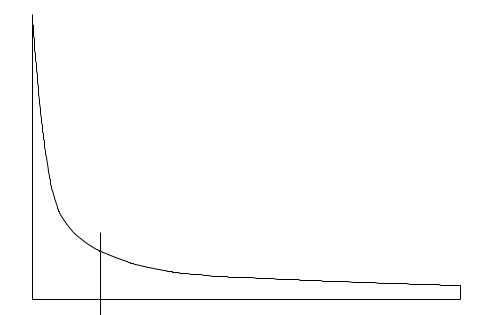
\includegraphics[width=8cm]{long-tail}
				\centering
				\caption{Fenómeno \textit{long--tail}}
			\end{figure}
			
		\subsubsection{Creando la matriz de utilidad}
			Como se desarrolló anteriormente, todo sistema de recomendación debe ser capaz de almacenar las preferencias de ciertos usuarios acerca de ciertos ítems. Para ésto, la estructura tradicional utilizada es la llamada matriz de utilidad. Ahora, ¿cómo se logra \enquote{llenar} ésta matriz?. Obtener información con la cual construir la matriz de utilidad es usualmente difícil. Sin embargo, existen ciertos enfoques para descubrir los valores con los cuales los usuarios califican los ítems:
			\begin{itemize}
				\item Pedir a los usuarios que califiquen ítems. Este enfoque es limitado ya que, por lo general, los usuarios no tienden a responder.
				\item Obtener conclusiones mediante el comportamiento del usuario. Si el usuario compra un ítem en Amazon, mira una película en YouTube, o lee una noticia, podemos decir que al usuario le \enquote{gusta} éste ítem. Este sistema de \textit{rating} tiene sólo un valor asociado: 1 significa que al usuario le \enquote{gusta} el ítem. Muchas veces, tambíen, nos encontramos con matrices de utilidad las cuales contienen valores 0's en vez de espacios en blanco. Esto quiere decir que el usuario no ha visto o comprado el producto. En éstos casos, un valor 0 no es menor que un valor 1; no es una calificación de \textit{rating}.
			\end{itemize}
			
	\subsection{Sistemas recomendadores basados en contenido}
		% Lucho
		
		En ésta sección se desarrollará una de las dos indentificables arquitecturas de sistemas de recomendación: aquellas basadas en contenidos. Como vimos anteriormente, los sistemas recomendadores basados en contenidos se enfocan principalmente en las propiedades de los ítems para, luego, computar similitudes entre pares de éstos.
		
		\subsubsection{Pefil de los ítems}
			Los sistemas basados en contendio deben crear un \textit{perfil} para cada ítem. Razonablemente, un perfil de un ítem es un \textit{conjunto} de características (propiedades) importantes las cuales representan al ítem. Como ejemplo introductorio, consideremos las características más importantes acerca de una película que, además, deben ser relevantes en un sistema recomendador:
			\begin{itemize}
				\item El conjunto de actores. Algunas personas prefieren aquellas peliculas las cuales trabajen sus actores favoritos.
				\item El director. Algunas personas, al elegir una película, consideran quién la ha dirigido.
				\item El año en el cual la película se estrenó. Algunas personas son amantes de películas viejas, mientras que otros las prefieren actuales.
				\item El género. Existen personas que prefieren comedias ante que dramas.
			\end{itemize}
			De todas las anteriores, el género es un concepto impreciso; es decir, es exclusivamente la opinión de una o varias personas que  hayan realizado la crítica a la película.
		
		\subsubsection{Extrayendo características de documentos e imágenes}
			Como sabemos, existen diversas \enquote{clases} de ítems. En éste capítulo consideraremos dos de ellas: colecciones de documentos e imágenes. De cada una de éstas clases de ítems debemos ser capaces de extraer características de los mismos para, luego, construir su correspondiente perfil. \par
			
			Existen muchos tipos de documentos para los cuales los sitemas de recomendación pueden ser útiles. Como sabemos, todos los días se publican miles de artículos los cuales, obviamente, no podemos leer. Un sistema recomendador puede sugerir aquellos artículos los cuales un usuario podría estar interesado. Pero, ¿cómo, éstos sistemas, pueden distringuir entre artículos?. Desafortunadamente, los artículos no tienen herramientas accesibles para saber (mediante, por ejemplo, una llamada a función) sus características y propiedades; como bien detallamos en el ejemplo anterior acerca de las características de una película. Por lo tanto, una forma de obtener información acerca de éstos documentos es mediante las técnicas de recuperación de información que estudiamos a lo largo de la monografía. En resumen:
			\begin{enumerate}
				\item Procesamiento de texto:
					\begin{enumerate}
						\item Obtener la secuencia de caracteres.
						\item \textit{Tokenization}.
						\item Eliminar \textit{stop words}.
						\item Normalización.
					\end{enumerate}			
				 \item Obtener los términos más frecuentes de cada documento. Estos tienden a expresar, de alguna manera, acerca de qué trata el documento.					
			\end{enumerate}
			Luego, podemos considerar como \textit{características} de un documento los $n$ términos más frecuentes computados en el paso 2 de la lista anterior. Es posible tomar $n$ de cada documento; es decir, $n$ fijo. También podemos tomar, del conjunto de todos los términos más frecuentes de un documento, sólo aquellos que superen cierta cota. Intuitivamente, decimos que éstos términos son los que expresan las principales ideas del documento. En un artículo de noticias podemos esperar que los términos con mayor frecuencia incluyan los nombres de las personas \enquote{involucradas} en el artículo, ubicación del evento, y demás. Uno de los métodos para medir la similitud entre documentos es la distancia del coseno (vista en el Capítulo 5): representamos cada documento como un vector $\vec{v}$ donde $\vec{v}[t] = 1$ si sólo si el término t es un término de alta frecuencia (es decir, pertenece al conjunto de los términos más frecuentes del documento en cuestión) dentro del documento, y $\vec{v}[t] = 0$ en otro caso. Como es de esperar, los vectores que representen los dos documentos de entrada para computar la similitud del coseno, tendrán mas componentes 0's que 1's; pero no impacta en el valor del producto escalar. \par
			
			Como bien se detalló, documentos de texto e imágenes son dos de los tipos de ítems mas compunes. Ahora, ¿cómo obtenemos características y propiedades acerca de una imagen?. Las imágenes son típicamente un array de píxeles, que no nos indican nada útil acerca de qué trata la imagen. Sí es posible calcular ciertas propiedades acerca de los píxeles, como por ejemplo el promedio total de la \enquote{cantidad} de negro en la imagen; pero pocos usuarios buscan específicamente imágenes de un determinado color. Una forma de solucionar éstos problemas es invitando a usuarios a etiquetar (\textit{tag}, en ingĺés) imágenes ingresando palabras o frases que la describan. Esta técnica se utiliza también en todos aquellos ítems los cuales no se tiene una idea clara sobre cómo, mediante sus estructuras de datos correspondientes, obtener características de los mismos. Por lo tanto, una imagen la cual pondera el color rojo podría ser etiquetada como \enquote{anochecer en Rosario}. Las etiquetas son explotadas en sistemas de recomendación. Sólo ocurre el problema que, muchas veces, los usuarios no se toman el trabajo de realizar el etiquetado de ítems.
			
			\subsubsection{Representación de perfiles de ítems}
				Todo sistema de recomendación basado en contenido debe ser capaz de poder representar, de alguna forma, sus dos principales entidades: ítems y usuarios. La representación de ítems debe contener los pares característica--valor, mientras que la representación de la entidad usuario debe resumir las preferencias del mismo (basadas en la matriz de utilidad). \par
				
				En la sección anterior se propuso una forma de representar ítems: un vector de sólo 0's y 1's, donde un 1 representa un término de alta frecuencia en el documento. Esta representación es trivial debido a que nos enfocamos en documentos de texto; es decir, todos los componentes del vector anteriormente mencionado representa un término dentro del documento. Todo sistema recomendador debe ser capaz de representar cualquier clase de ítem. Es realmente fácil cuando se tienen que representar características que son conjunto de valores discretos. Para ejemplificar lo anterior, tomemos el ejemplo de las películas. Una de las características de una película es el conjunto de actores los cuales trabajaron en ella. Este conjunto, obviamente, es un conjunto discreto. Imaginemos que hay un componente por cada actor, donde el valor 1 representa que el actor trabajó en la película en cuestión, y 0 representa el caso contrario. \\
				Ahora, ¿qué sucede con aquellas características que no pueden ser representadas por vectores booleanos?. Estas características se denominan \textit{numéricas}. Por ejemplo, la calificación de una película; la cual es un número real. No tiene sentido tener un componente para cada uno de las posibles calificaciones. Estas características deben ser representadas por componentes indiviudales. Cabe destacar que no existe ningún daño si alguno de los componentes de un vector toman valores booleanos (1's ó 0's) y otros toman valores reales o enteros: es posible computar la distancia del coseno entre vectores.
				\begin{quote}
					\textbf{Ejemplo 8.2}. A modo de ejemplo, sean dos películas $A$ y $B$ en las cuales sólo se representan el conjunto de actores y la calificación promedio. Supongamos que cada película tiene cinco actores cada una.
					
					\begin{tabular}{llllllllll}
						Película $A$: & 0 & 1 & 1 & 0 & 1 & 1 & 0 & 1 & 3$\alpha$ \\
						Película $B$: & 1 & 1 & 0 & 1 & 0 & 1 & 1 & 0 & 4$\alpha$
					\end{tabular} \\	
					
					De la representación anterior podemos concluir que la película $A$ tiene una calificación promedio de 3 puntos, mientras que $B$ tiene una calificación promedio de 4 puntos. Vemos también que ambas películas comparten dos actores. \\
					
					Razonablemente, existen \enquote{infinitos} componentes adicionales cada uno con valor 0 en cada vector. Estos representan aquellos actores que no trabajan en ninguna de las dos películas. La distancia del coseno no es afectada por componentes nulos (es decir, con componentes con valor 0). \\
					
					Como vemos, el último componente indica la calificación promedio de la película. Este es afectado por un escalar desconocido $\alpha$. Ahora, computemos la similitud del coseno entre éstos dos vectores. El producto escalar (también conocido como producto interno) entre ambos vectores es $2 + 12\alpha^2$, y las longitudes de los vectores son $\sqrt{5 + 9\alpha^2}$ y $\sqrt{5 + 16\alpha^2}$, respectivamente. Luego, la distancia del coseno entre las representaciones de las películas $A$ y $B$ es:
					\begin{equation}
							\frac{2 + 12\alpha^2}{\sqrt{25 + 125\alpha^2 + 144\alpha^4}}
					\end{equation}
				\end{quote}
				
				Si tomamos $\alpha = 1$ (es decir, sin alterar las calificaciones), la similitud entre los dos vectores es 0,816. Mientras que si tomamos $\alpha = 2$, el coseno es 0,940; es decir, los vectores parecen más cercanos en dirección. Ahora, si usamos $\alpha = 1/2$, luego, el coseno es 0,619, logrando que la similitud entre los vectores sea bastante diferente. No es posible saber qué valor de $\alpha$ es el \enquote{correcto}, pero desde ya podemos visualizar cómo afecta escalar su valor y, por lo tanto, cómo afecta nuestra decisión sobre cuán similares son los ítems.
				
			\subsubsection{Representación de perfiles de usuario}
				Ahora, necesitamos definir una estructura para representar el perfil de un usuario. Debemos crear vectores con los mismos componentes que utilizamos en la sección anterior para representar el perfil de un ítem. \par
				
				Recordemos que la matriz de utilidad representa la \enquote{conexión} entre usuarios e ítems. En ella, pueden existir componentes con valor 1 representando compra de usuarios o pueden existir valores numéricos arbitrarios representando la calificación que el usuario brindó al ítem en particular. \par
				
			\subsubsection{Recomendando ítems a usuarios basado en contenido}	
				Finalmente, teniendo a disposición los vectores de los usuarios y los ítems, podemos estimar el grado de preferencia de un usuario hacia cierto ítem computando la distancia del coseno entre ambos vectores.
				
			\subsubsection{Limitaciones}
				Los sistemas recomendadores basados en contenidos presentan varias limitaciones. Entre las más importantes se encuentran:
				\begin{itemize}
					\item Análisis de contenido limitado. Estos sistemas son difíciles de implementar cuando los ítems son archivos multimedia (imágenes, videos). Una forma de sortear ésta limitación es mediante el uso de etiquetas, como estudiamos anteriormente.
					\item Sobre--especialización: los ítems recomendados a un usuario son limitados a aquellos que son similares a los cuales el usuario ya calificó.
					\item Problema del nuevo usuario (\textit{cold start problem}). Para que un sistema de recomendación basado en contenido entienda las preferencias de un usuario, el usuario debe calificar un número suficiente de ítems. Por lo tanto, éstos sistemas fallan al recomendar ítems para usuarios los cuales han calificado pocos ítems.
				\end{itemize}
			
	\subsection{Sistemas recomendadores basados en filtrado colaborativo}
	% Estani
	
\section{Sistemas de recomendación sociales}
	\subsection{Introducción}
		Con el desarrollo de la World Wide Web, la información ha ido incrementando a escales sin precedentes. Como estudiamos al comienzo de éste capítulo, lo anterior trae consecuencias a la hora de buscar información en la Web ya que lo usuarios se encuentran ante millones de fuentes de información. Para ejemplificar lo anterior, si ingresamos el término \textit{computadora} en Amazon, devolverá millones de productos. Por lo tanto, hemos visto que un sistema recomendador es esencial en empresas de éste estilo (es decir, comercios on--line): éstos sistemas intentan abordar el problema de sobrecarga de información sugeriendo sólo aquella que son de potencial interés para los usuarios on--line. Un buen sistema recomendador puede llevar al éxito a un comercio on--line. \par
		
		El incremento de las redes sociales (como Facebook y Twitter, entre otras) brindan a usuarios diferentes herramientas para comunicarse digitalmente y permitir que éstos compartan ideas y opiniones con otros usuarios compartidos. Es decir, las redes sociales emergieron para, de alguna forma, \enquote{potenciar} la vida social de las personas. Las preferencias de un usuario es similar o influenciada por sus amigos socialmente conectados. Esto puede ser explicado por teorías como homofilia e influencia social. Se denomina homofilia a la tendencia de las personas a relacionarse con personas que se parecen a ellas debido a diferentes atributos como pueden ser creencias, clase social, educación, edad, etc. Es decir, usuarios con preferencias similares tienden a estar conectados. Mientras que la influencia social indica que los usuarios que están conectados tienden a tener preferencias similares. En el transcurso de nuestras vidas, las personas tienden a consumir productos los cuales fueron sugeridos por aquellas personas las cuales estamos conectados socialmente mediante alguna forma (amistad, parentesco, entre otras). Por lo tanto, las relaciones sociales pueden ser explotadas para mejorar el rendimiento de sistemas recomendadores tradicionales \cite{tang2013}.
		
	\subsection{Definición de recomendador social}
		Existen diversas definiciones sobre un recomendador social, pero ninguna comúnmente aceptada. Aquí daremos dos de ellas:
		\begin{itemize}
			\item \enquote{La recomendación social es cualquier recomendación con relaciones sociales on--line como entrada adicional; es decir, aumentar el motor de cualquier sistema de recomendación tradicional con señales sociales} \cite{king2010}. \\
				En ésta definición, las preferencias de los usuarios tienden a ser similares o a estar influenciadas por sus conexiones sociales. Bajo las suposiciones anteriores, las relaciones sociales ayudan y mejoran el rendimiento de recomendación. Algunos sistemas que se basan en la definición anterior son TidalTrust, MoleTrust, SoRec, SocialMF, SoReg y LOCALBAL.
			\item \enquote{Un sistema recomendador social es un sistema recomendador (tradicional) que se dirijen (o tienen como destino) a medios sociales} \cite{guy2011}. Esta es una definición mucho más amplia que la anterior ya que las fuentes de entrada del sistema no sólo están limitados a relaciones sociales on--line sino que también incluyen todo otro tipo de fuente social disponible como interacciones de usuarios y comportamiento de usuarios.
		\end{itemize}
		
		En éste capítulo utilizaremos la primera definición y presentaremos algunos sistemas recomendadores sociales, basados en ésta definición, en estado del arte.
	
	\subsection{Un modelo para sistemas recomendadores sociales}
		Como sabemos, en sistemas de recomendación sociales, además de la matriz de utilidad que desarrollamos al comienzo del capítulo, los usuarios se pueden conectar con otros usuarios. Notamos $R$ a la matriz de utilidad ($R$, por \textit{rating}). Ahora, sea $T \in \mathbb{R}^{n \times n}$ la matriz que denota las relaciones usuario--usuario, donde $T_{i,j} = 1$ si el usuario $u_j$ se encuentra conectado socialmente con el usuario $u_i$, y 0 en caso contrario. Esta matriz $T$ es la que llamamos fuente social y es la entrada adicional de un sistema recomendador tradicional para \enquote{transformarlo} en un sistema recomendador social. \par
		
		 En los sistemas recomendadores tradicionales, se asume que los usuarios son independientes. Pero como hemos desarrollado al comienzo de la sección, los usuarios on--line están conectados entre ellos mediante distintos tipos de relaciones (amistad, parentesco, etc). Luego, en un sistema recomendador social, los usuarios están correlacionados en lugar de ser independientes. La Figura \ref{fig:sistema-recomendador-tradicional-social} ejemplifica lo anterior.
		 
		 %% Figura 1 (tang2013)
		 \begin{figure}
			\centering
			\begin{subfigure}[b]{0.5\linewidth}
				\centering
				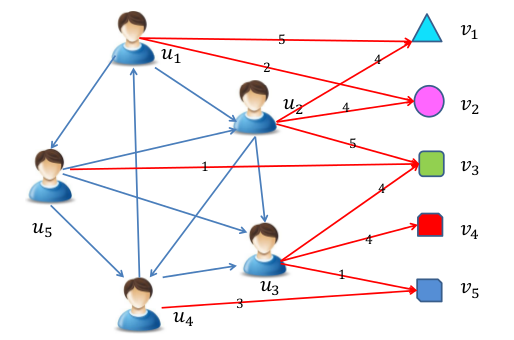
\includegraphics[width=8cm]{social-graph}
				\caption{Grafo de relaciones entre usuarios e ítems}
			\end{subfigure}
			
			\begin{subfigure}[b]{0.5\linewidth}
				\centering
				\[
			R =
			\kbordermatrix{
				& v_1 & v_2 & v_3 & v_4 & v_5 \\
			u_1 & 5   &     &  2  &     &     \\
			u_2 & 4   &  4  &  5  &     &     \\
			u_3 &     &     &  4  &  4  &  1  \\
			u_4 &     &     &     &     &  3  \\
			u_5 &     &     &  1  &     &     
			}
			\]
				\caption{Un sistema recomendador tradicional}
			\end{subfigure}
			
			\begin{subfigure}[b]{0.5\linewidth}
				\centering
				\[
			R =
			\kbordermatrix{
				& v_1 & v_2 & v_3 & v_4 & v_5 \\
			u_1 & 5   &     &  2  &     &     \\
			u_2 & 4   &  4  &  5  &     &     \\
			u_3 &     &     &  4  &  4  &  1  \\
			u_4 &     &     &     &     &  3  \\
			u_5 &     &     &  1  &     &     
			}
			\]
			\\
			\[
			T =
			\kbordermatrix{
				& u_1 & u_2 & u_3 & u_4 & u_5 \\
			u_1 & 0   &  1   &  0  &  0   & 1    \\
			u_2 & 0   &  0  &  1  &  1   &  0   \\
			u_3 & 0    & 0    &  0  &  0  &  0  \\
			u_4 & 1   &  0   &  1   &  0   &  0  \\
			u_5 & 0    & 1    &  1  &  1   &  0   
			}
			\]
				\caption{Sistema recomendador social, donde R es la matriz de utilidad y la matriz T representa las relaciones sociales entre usuarios}
			\end{subfigure}
			
			\caption{Relación entre usuarios socialmente correlacionados y calificaciones de ítems}
			\label{fig:sistema-recomendador-tradicional-social}
		\end{figure}
	
	\subsection{Sistemas recomendadores sociales existentes}
		%% Sólo vamos a estudiar "Model based social recommender systems" (véase tang2013)
		
		Para introducir algunos sistemas existentes (en estado del arte), debemos volver hacia atrás y recordar, brevemente, acerca de sistemas recomendadores (tradionales) basados en filtrado colaborativo. El filtrado colaborativo es la técnica más popular en la actualidad para desarrollar sistemas recomendadores \cite{ullman2014}. En vez de utilizar características (propiedades) de ítems para determinar su similitud, los sistemas basados en filtrado colaborativo se enfocan en la similitud entre usuarios. Es decir, cuando el sistema recomienda ítems a un usuario $u$, lo realiza \enquote{estudiado} a aquellos usuarios similares a $u$ y, por lo tanto, recomendando ítems los cuales éstos usarios \enquote{aprecian} (es decir, han otorgado una buena calificación). Estos sistemas parten de la suposición de que si hay usuarios que compartieron los mismos gustos en el pasado, entonces también los compartirán en el futuro. Luego, todo se reduce a computar la similitud entre usuarios, utilizando los vectores de \textit{rating} de la matriz de utilidad, anteriormente notada $R$. Sabemos que para calcular la similitud entre vectores existen diversos métodos; entre ellos, la similitud del coseno. \par
		
		Los sistemas recomendadores basados en filtrado colaborativo son, también, los sistemas más populares para implementar sistemas recomendadores sociales. Por lo tanto, los utilizaremos en lo que resta del capítulo. \par
		
		Como vimos anteriormente, los sistemas recomendadores sociales poseen dos entradas de datos: la información de calificaciones usuario--item (matriz de utilidad, $R$) y la información sobre relaciones sociales entre usuarios (matriz anteriormente notada como $T$). Por lo tanto, un sistema recomendador social basado en filtrado colaborativo tiene dos partes \cite{tang2013}:
		\begin{quote}
			sistema recomendador social basado en filtrado colaborativo = modelo básico de filtrado colaborativo + modelo social de información
		\end{quote}
		
		Recordemos el funcionamiento de un sistema recomendador tradicional basado en filtrado colaborativo cuando se desconoce una calificación de cierto usuario $u_i$ a cierto ítem $i_j$; es decir, cuando se desconoce $R_{i,j}$. Este valor se computa de la siguiente forma:
		\begin{enumerate}
			\item Se obtiene el conjunto de todos los usuarios similares a $u_i$. Lo notamos $N$.
			\item Se computa el valor de $R_{i,j}$ como el promedio de las calificaciones que otorgaron los usuarios en $N$ al ítem $i_j$.
		\end{enumerate}
		
		Ahora, dado que en un sistema recomendador social tenemos, además, información social acerca de los usuarios, ¿cómo se computa un valor desconocido dentro de la matriz $R$?. El procedimiento es análogo al anterior salvo que se tienen en cuenta las relaciones sociales entre usuarios: se debe obtener un conjunto, $N^+$, el cual obtiene información social acerca del usuario como también información de \textit{rating}. \par
		
		Existen diferentes formas de obtener el conjunto $N^+$. En ésta sección presentaremos algunos algoritmos en estado del arte: TrustWalker \cite{jamali2009}... (agregar uno o dos mas de los nombrados).
		
		\subsubsection{TrustWalker}
			Como hemos visto, el filtrado colaborativo es el método más utilizado para crear sistemas recomendadores. Es muy efectivo cuando los usuarios ya han calificado suficientes ítems, para tener calificaciones en común con otros usuarios. Pero el filtrado colaborativo tiene la siguiente gran desventaja: realiza un desempeño pobre en usuarios nuevos; es decir, en aquellos los cuales sólo han calificado \textit{pocos} ítems. Este problema se llama \textit{cold--start problem}. Los métodos de recomendación basados en confianza (trust--based recommendation methods, en inglés) suman la información de una red de confianza entre usuarios y, por lo tanto, pueden lidiar con el problema anterior ya que \enquote{consultan}, sobre determinado ítem(s), a aquellos usuarios que considera de confianza (decimos que $u_i$ es de confianza de $u_j$ si y sólo si ambos usuarios están relacionados socialmente de alguna forma: amistad, parentesco, etc). \par
			
			Utilizando una red de confianza, mejora el procedimiento de sistemas recomendadores basados en filtrado colaborativo. Sin embargo, en el proceso de recorrer la red de confianza, cuanto más nos alejamos del usuario origen $u$, la confianza entre éstos usuarios y el origen será bastante débil y sus calificaciones (\textit{ratings}) no serán confiables. Lo que implica que debemos usar aquellas calificaciones de usuarios en el \enquote{vecindario} (es decir, aquellos usuarios que están directamente correlacionados socialmente). Con éste motivo nació el algoritmo TrustWalker. El algoritmo propone, dada la red de confianza (la matriz $T$ anteriormente definida y también usualmento llamado \textit{social graph}) realizar una caminata aleatoria la cual combina métodos de recomendación basados en confianza y basados en similitud de ítems (filtrado colaborativo).
			
			\textbf{Definición del problema}. En un sistema recomendador (tradicional), llamemos al conjunto de usuarios $U = \{u_1,...,u_N\}$ y al conjunto de ítems $I = \{i_1,...,i_M\}$. Sabemos que cada usuario califica a un cierto conjunto de ítems, el cual lo notaremos como $RI_u = \{i_{u_1},...,i_{u_k}\}$. Recordemos también que $R_{u,i}$ es la calificación que un usuario $u$ otorga a un ítem $i$, donde $R$ es la matriz de utilidad definida al comienzo de capítulo. Como vimos, éstos valores pueden ser números reales o, generalmente, números enteros pertenecientes al conjunto [1,5]. Los sistemas recomendadores basados en confianza, además de la matriz de utilidad, poseen como entrada una red de confianza. Si el usuario $u$ confía en el usuario $v$ (es decir, ambos usuarios están directamente conectados socialmente), luego $T_{u,v} = 1$, y $T_{u,v} = 0$ en caso contrario. $T$ es la matriz que denota las relaciones usuario--usuario que definimos cuando se introdujo la definición de un sistema recomendador social. Definimos $TU_u = \{v \in U | T_{u,v} = 1\}$ al conjunto de usuarios que están directamente conectados con $u$. Esto da motivo para representar a la red de confianza como un grafo $G = <U,TU>$ donde $TU = \{(u,v) | u \in U, \ v \in TU_u \}$. \\
			Recordemos que la mayoría de los valores de la matriz de utilidad, $R$, son desconocidos: dado un usuario $u$ y un ítem $i$, para el cual se desconoce la calificación de $u$ a $i$, es trabajo del sistema recomendador \enquote{predecir} $R_{u,i}$ donde llamamos usuario \textit{fuente} a $u$ e ítem \textit{objetivo} al ítem $i$. \\
			La mayoría de los sistemas de recomendación tradicionales (aquellos implementados mediante métodos de filtrado colaborativo) estiman el valor $R_{u,i}$ basados en calificaciones a $i$ de usuarios similares a $u$. Un sistema recomendador basado en una red de confianza, para predecir el \textit{rating} $R_{u,i}$ pregunta a aquellos usuarios de confianza conectados directamente a $u$ si conocen la calificación del ítem en cuestión, $i$. Si es así, la devuelven. En caso contrario, el sistema pregunta recursivamente a los vecinos directos de $u$. Las calificaciones obtenidas son acumuladas para, luego, producir la recomendación. \\
			En resumen, una red social provee una fuente independiente de información que puede ser explotada para mejorar los resultados y la calidad de recomendación. Esta información, en particular, ayuda a combatir el \textit{cold--start problem}. El objetivo de un recomendador como el que estamos definiendo es predecir calificaciones desconocidas basadas en calificaciones de \enquote{amigos} confiables. \par
			
			\textbf{Definiendo el modelo de TrustWalker}. El principal desafío en un sistema recomendador basado en una red de confianza es decidir cuán lejos explorar ésta red. Cuanto más lejos se explora, se tiene más probabilidades de encontrar un usuario que haya calificado el ítem en cuestión pero, a la vez, sus calificaciónes son menos confiables. TrustWalker se basa en la siguiente observación: las calificaciones expresadas por usuarios \textit{fuertemente} confiables en ítems similares, son más confiables que aquellas calificaciones expresadas por usuarios lejos del \enquote{vecindario} (es decir, aquellos usuarios no \textit{fuertemente} conectados socialmente) en el mismo ítem. El algoritmo combina métodos de recomendación basados en redes de confianza y métodos de recomendación de ítems similares (filtrado colaborativo). \\
			Luego, se propone un modelo de \enquote{caminata} aleatoria, llamada TrustWalker, que considera no sólo calificaciones del ítem objetivo, sino también aquellas calificaciones de ítems similares. Básicamente, el algoritmo consiste en dos componentes:
			\begin{itemize}
				\item La caminata aleatoria en la red de confianza, la cual realiza la búsqueda en la red.
				\item La selección de ítems. Este considera las calificaciones de ítems similares para evitar que la caminata aleatoria no recorra muy profundamente la red de confianza.
			\end{itemize}
			
			\textbf{Caminata aleatoria}. La caminata aleatoria comienza desde un usuario origen $u_0$. En cada paso $k$ de la caminata, nos encontramos en un cierto nodo $u$. Si éste mismo usuario, $u$, tiene una calificación para el ítem objetivo $i$, luego se detiene la caminata y el algoritmo devuelve $R_{u,i}$ como resultado de la caminata. En el caso de que $u$ no tenga una calificación para el ítem objetivo $i$, tenemos dos opciones:
			\begin{itemize}
				\item Con probabilidad $\phi_{u,i,k}$, no continuamos con la caminata aleatoria. Permanecemos en el nodo $u$ y aleatoriamente seleccionamos uno de los ítems, $j$, similar a $i$ calificado por $u$ y se devuelve $R_{u,j}$.
				\item Con probabilidad $1 - \phi_{u,i,k}$, continuamos la caminata aleatoria hacia otro usuario $v$ quien es uno de los vecinos directamente correlacionados ($v \in TU_u$).
			\end{itemize}
			
			Ahora, veamos cómo, el algoritmo, procede en las distintas posibilidades. Si se decide continuar la caminata aleatoria estando en el nodo $u$, debemos seleccionar un vecino de los vecinos directamente correlacionados de $u$ para proseguir con la caminata hacia ése usuario. Definimos $S_u$ a la variable aleatoria para seleccionar un usuario $v$ del conjunto, anteriormente definido, $TU_u$:
			\begin{equation}
				P(S_u = v) = \frac{T_{u,v}}{\sum_{w \in TU_u} T_{u,w}} = \frac{1}{|TU_u|}
			\end{equation}
			
			Finalmente, se debe analizar el caso restante. Con probabilidad $\phi_{u,i,k}$, si decidimos detener la caminata aleatoria en el usuario $u$, debemos seleccionar uno de los ítems calificados por $u$ que sea similar al ítem objetivo $i$. Para ésto, se debe definir una medida de similitud entre ítems, $sim(i,j)$, la cual se desarrollará más adelante. Luego, para cada ítem $j \in RI_u$, se asigna una probabilidad de selección proporcional a la similitud entre $i$ y $j$, la cual \cite{jamali2009} define así:
			\begin{equation}
				P(Y_{u,i} = j) = \frac{sim(i,j)}{\sum_{l \in RI_u} sim(i,l)}
			\end{equation}
			$Y_{u,i}$ es la variable aleatoria para seleccionar un ítem $j$ entre todos los demás ítems calificados por $u$ mientras encuentra un ítem similar al objetivo, es decir, $i$. Como resultado final de la caminata aleatoria, el algoritmo devuelve $R_{u,j}$. \par
			
			En TrustWalker, para medir la similitud entre dos ítems $i$ y $j$, se utiliza la Correlación de Pearson, la cual se nota como $corr(i,j)$:
			\begin{equation}
				corr(i,j) = \frac{\sum_{u \in UC_{i,j}} (R_{u,i} - \overline{R}_u)(R_{u,j} - \overline{R}_u)}{\sqrt{\sum_{u \in UC_{i,j}} (R_{u,i} - \overline{R}_u)^2}\sqrt{\sum_{u \in U} (R_{u,i} - \overline{R}_u)^2}}
			\end{equation}		
			$UC_{i,j}$ es el conjunto de usuarios en común que han calificado ambos ítems $i$ y $j$. $\overline{R}_u$ representa el promedio de expresados por el usuario $u$. \\
			
			El tamaño de $UC_{i,j}$ es importante ya que, por ejemplo, si $corr(i,j) = corr(i,l)$ pero $|UC_{i,j}| > |UC_{i,l}|$, entonces $i$ y $j$ han sido calificado por más usuarios en común. Luego, la correlación entre los ítems es mayor y $sim(i,j)$ debe ser mayor que $sim(i,l)$. \cite{jamali2009} propone la similitud entre dos ítems $i$ y $j$, como sigue:
			\begin{equation}
				sim(i,j) = \frac{1}{1 + e^{-\frac{|UC_{i,j}|}{2}}} \times corr(i,j)
			\end{equation}
			
			\begin{quote}
				\textit{Función sigmoide}. Una función sigmoide es una función real diferenciable acotada que se define para todos los valores reales de las entradas y tiene una derivada positiva en cada punto \cite{han1995}.
				
				\begin{equation}
					S(t) = \frac{1}{1 + e^{-t}}
				\end{equation}
				
				\begin{figure}[h]
					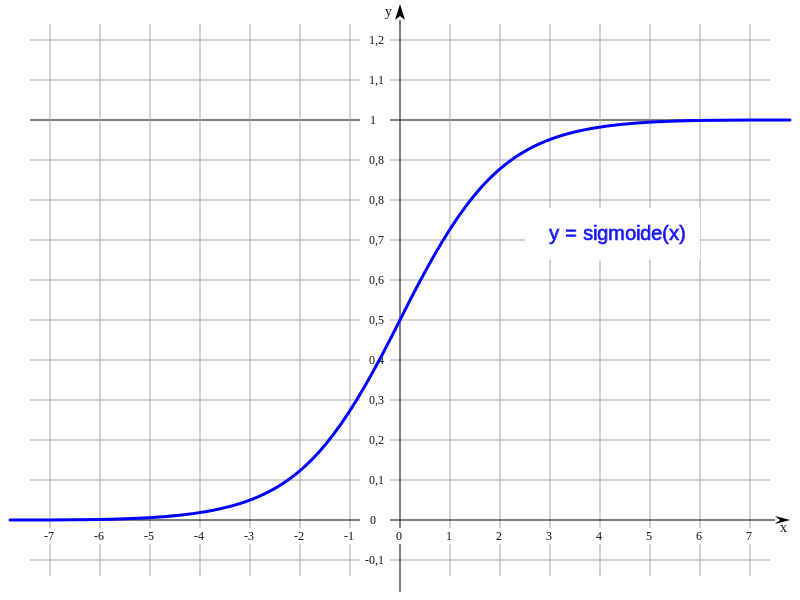
\includegraphics[width=8cm]{sigmoide}
					\centering
					\caption{Función sigmoide}
				\end{figure}
				
				Esta función permite describir procesos la evolución de muchos procesos naturales y curvas de aprendizaje de sistemas complejos. Estos tienen una progresión temporal desde unos niveles bajos al inicio, hasta hacercarse a un \enquote{climax} transcurrido un cierto tiempo.
			\end{quote}
			
		Aquí, en TrustWalker, la función simoide se utiliza para evitar favorecer demasiado el tamaño del conjunto $UC_{i,j}$ y mantener la similitud en el rango [0,1].
			 